% main.tex — the one canonical entry point for the DNP3 timing-obfuscation manuscript.
%
% Build (from paper/rewrite/):   ./pipeline/build.sh        -> pipeline/build/main.pdf + gate
%        or, standalone:         tectonic -X compile main.tex
%
% Sections live in sections/ in the order the manuscript uses. Writing rules:
% pipeline/DR_LIN_WRITING_GUIDE.md. Claim boundaries: ../../defense4/timing/CLAIMS_AND_LIMITATIONS.md.
%
\documentclass[conference]{IEEEtran}
\IEEEoverridecommandlockouts

\usepackage{cite}
\usepackage{amsmath}
\usepackage{graphicx}
\usepackage{booktabs}
\usepackage{array}
\usepackage{url}
\usepackage[T1]{fontenc}
\usepackage{textcomp}
\usepackage{upquote}

\newcommand{\code}[1]{\texttt{#1}}
% A missing figure PDF renders as a labelled box, never as a compile error or a black region.
\newcommand{\figplaceholder}[1]{\fbox{\parbox[c][3.3cm][c]{0.9\columnwidth}{\centering\footnotesize\ttfamily [FIGURE PLACEHOLDER]\\[3pt]\normalfont\itshape #1}}}

\begin{document}

\title{Programmable In-Network Timing Obfuscation for DNP3}

% Authors confirmed by Philip on 2026-08-26 (Philip Akekulip, Hui Lin). Affiliation: University
% of Nevada, Reno, the DECPS lab (supported by the group's DefRec/RAINCOAT records and the lab
% path on the switch). Email addresses are not in the repository and are left as visible
% placeholders; fill them in before submission.
\author{\IEEEauthorblockN{Philip Akekulip and Hui Lin}
\IEEEauthorblockA{University of Nevada, Reno\\
\{[email pending], [email pending]\}}}

\maketitle

\begin{abstract}
An adversary watching a power-grid control network can tell which device it is looking at from
how long that device takes to answer, because vendors implement the same function differently.
Hiding that timing is challenging. The relay cannot be modified, and existing traffic obfuscation
was built for a different feature: it reshapes flow-level sizes and inter-packet times, whereas
the feature that identifies the device here is one interval inside a single transaction. It also
hides the packets it adds behind encryption, which these plaintext networks do not have.

To change the timing without touching either endpoint, we put the defense in the network. A
programmable switch in front of the outstation holds the device's acknowledgment and its
response, and releases each at a deadline computed from the same instant, the moment the outstation
acknowledges the request. Neither release depends
on how long the device took, so the interval an observer measures is a value the operator sets.
The switch forwards the packets it received, so both endpoints run unmodified and no DNP3 byte
changes.

We implement this on an Intel Tofino-1 and evaluate it against one physical SEL-751A protective
relay. The measured interval settles on the configured value: its median is the configured 4~ms,
its interquartile range falls by more than two orders of magnitude, and its sample variance falls
from 6.808 to 0.394~ms$^2$. A classifier trained on that interval before deployment is left at
chance across the three transaction classes. An adversary who retrains recovers much of that from
a second interval we do not target, and that residual bounds what the framework achieves. The
evaluation covers transaction-class timing for a single device; we do not measure confusion
between device models, and we do not claim the feature is removed for an adversary who accumulates many
observations.
\end{abstract}


\begin{IEEEkeywords}
DNP3, device fingerprinting, timing side channels, traffic obfuscation, programmable switches,
industrial control systems.
\end{IEEEkeywords}

% Authors' Introduction, supplied 2026-08-26. Paragraphs 1-3 are kept verbatim apart from
% added citations and the corrected DNP3 framing/CRC explanation. The contribution
% list was rewritten to verb-led form without a firstness claim. See
% pipeline/reports/LIN_TEXT_CHANGELOG.md.
\section{Introduction}
\label{sec:intro}

Device fingerprinting has been an essential step in cyber reconnaissance, allowing adversaries
to reveal unique features of target networks and design effective, stealthy attack strategies.
These techniques are becoming increasingly critical in industrial control systems (ICSs) such as
power grids, where adversaries often use IP-based control networks and computing devices within
as entry points to inflict physical damage. Consequently, fingerprinting shifts the focus from
visited websites and user biometric behavior to device models and types of control operations
that are critical to ICS attacks. In the 2015 attack that disrupted Ukrainian power grids and
the Stuxnet attack that disrupted Iranian nuclear power facilities, it is widely believed that
adversaries stay in their systems for at least 6 months to perform cyber
reconnaissance~\cite{leeAnalysisCyberAttack2016, langnerStuxnetDissectingCyberwarfare2011}.

To disrupt device fingerprinting, many studies present network traffic
obfuscation~\cite{wrightTrafficMorphingEfficient2009, dyerPeekaBooStillSee2012}. Because device
fingerprinting targeting general computing environments generally relies on network-level
features such as packet size and/or inter-packet latency observed from communication
patterns~\cite{sirinamDeepFingerprintingUndermining2018}, traffic obfuscation often focuses on
(i) padding and splitting network packets, which hide or change the distribution of network
packet sizes~\cite{wrightTrafficMorphingEfficient2009}, and (ii) delaying network packets and
adding dummy ones, which disrupt the inter-packet timing pattern~\cite{dyerPeekaBooStillSee2012,
caiSystematicApproachDeveloping2014}. Since manipulating communication networks can introduce
runtime overhead, recent works have begun to offload traffic obfuscation onto programmable
network switches, which change communication patterns at much higher line rates than
CPUs~\cite{meierDittoWANTraffic2022, wangMinosLightweightDynamic2025,
xieSecuritasDefendingTraffic2026}.

Unfortunately, these methods do not directly transfer device fingerprinting in ICS/SCADA
environments for two main reasons. First, the leaked features are different. General web traffic
obfuscation usually targets the flow level sizes and timing patterns~\cite{meierDittoWANTraffic2022}
whereas ICS device fingerprinting is carried by the response timing of the protocol exchanges,
which stays visible even when the payload is encrypted~\cite{formbyWhosControlYour2016}.
Secondly, adding bytes or cover packets is constrained in this setting in a way it is not on the
open Internet. A DNP3 link-layer frame carries a declared length and a cyclic redundancy check
(CRC) over each block of the frame~\cite{ieeeIEEEStandardElectric2012}, so bytes inserted at an
arbitrary offset change the framing the receiver parses. Making such an insertion valid requires
protocol-aware reconstruction of the frame and recomputation of its link-layer CRC blocks, which
is not what an opaque pad does. The outstation that would otherwise emit cover traffic is a
protective relay whose firmware cannot be modified, so a legacy relay cannot simply be made to
generate that traffic either. Consequently, a defense in this setting must hide the timing that
leaks even after encryption while changing no bytes.

In this paper, we present an in-network mechanism that normalizes an outstation's
fingerprintable features using the data plane of the Tofino programmable switch at the
outstation edge, without changing the endpoints or modifying the bytes of the DNP3 traffic. This
defense holds per transaction responses and releases them at configurable offsets so the
master-visible timing then becomes a policy value. The two timing features that Formby et
al.~\cite{formbyWhosControlYour2016} use for fingerprinting, the cross-layer response time of a
poll and the master-visible timing of a control command, are the two case studies through which
we show the framework working; they are not two separate systems. We implement the framework as
a P4 program on a single switch, evaluate it on a cyberphysical testbed, and make the following
contributions:
\begin{itemize}
  \item \textbf{Design an in-network timing-obfuscation framework} that replaces selected
    within-transaction timing features with configurable release-policy values, without
    modifying either endpoint and without changing the protected DNP3 bytes.
  \item \textbf{Implement the framework on an Intel Tofino-1} as a P4 program with a separate
    acknowledgment-anchored read lane and request-anchored control lane, bounded queues, and
    fail-open forwarding when a response arrives after its scheduled release.
  \item \textbf{Evaluate the framework against a physical SEL-751A relay} over 22 grouped
    collection runs, and report policy programmability, timing-feature suppression, the effect
    on a fixed transaction-class attacker, the leakage that remains against an adaptive
    attacker, and the latency the mechanism costs.
\end{itemize}

\section{Background and Motivation}
\label{sec:bg}

In this section we focus on the DNP3 transactions the paper covers, the features that leak from
them and how an adversary uses them in fingerprinting, and the opportunity that a programmable
data plane gives us to change the timing without touching the endpoints.

\begin{figure}[t]
\centering
\IfFileExists{figures/fig_ladder.pdf}{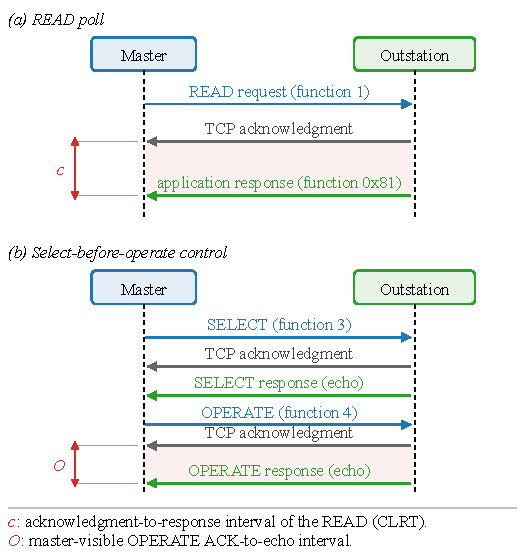
\includegraphics{figures/fig_ladder}}{\figplaceholder{DNP3 transaction ladder: (a) READ request, TCP ACK, application response; (b) SELECT, TCP ACK, SELECT response, OPERATE, TCP ACK, OPERATE response.}}
\caption{The DNP3 transactions the paper measures, as seen on the master-facing link; requests in
blue, transport-layer acknowledgments in grey, and application responses in green. (a) A READ
poll: the request, the outstation's transport-layer acknowledgment, and its application-layer
response. The interval $c$ between the acknowledgment and the response is the cross-layer
response time (CLRT). (b) A select-before-operate control: SELECT and OPERATE each produce an
acknowledgment and a solicited application response. The interval $O$ between the OPERATE's
acknowledgment and its solicited response is the master-visible OPERATE response-to-ACK interval.}
\label{fig:ladder}
\end{figure}

\textbf{The DNP3 read and control transactions.} DNP3 carries supervisory control and data
acquisition (SCADA) traffic over TCP between a master and an outstation~\cite{ieeeIEEEStandardElectric2012}.
The master polls the outstation with a READ request (function code 1), and the outstation
returns the requested measurements in an application-layer response (function code 0x81). A
control command, on the other hand, uses select-before-operate (SBO): the master first sends a
SELECT (function code 3) that names an output point, and the outstation returns a SELECT
application response; the master then sends an OPERATE (function code 4), which the outstation
confirms with a solicited OPERATE application response. A DNP3 control response repeats the
control object, but it is a solicited application response, not a distinct message type. Because DNP3 runs over TCP, every request is also
acknowledged at the transport layer before the application answers. As such, each transaction on
the wire is a request, a TCP acknowledgment that carries no DNP3 payload, and a DNP3 response, in
that order, as Figure~\ref{fig:ladder} shows. We use these terms consistently in the rest of the
paper: the acknowledgment is the TCP segment with the ACK flag that the outstation returns
first, and the response is the DNP3 application frame that follows it.

\textbf{Why the transaction timing is a fingerprint.} The acknowledgment is produced by the
outstation's TCP stack as soon as the request arrives, whereas the response is produced by its
application only after the device has done the work the request asks for. Consequently, the
interval between the two, the CLRT, reflects the outstation's internal processing rather than
the network path, and it differs between device models and between the kinds of work they do.
Formby et al.\ used it to tell device types and models apart in a substation network, and used
the time a device takes to complete a control operation as a second feature that reveals the
physical device behind the command~\cite{formbyWhosControlYour2016}. Our own measurements on a
physical SEL-751A relay show the same effect on one device: with no timing defense, the median
CLRT is 2.116~ms for a READ, 2.050~ms for a SELECT and 2.937~ms for an OPERATE, each with a long
tail, so the three transaction classes are already partly separable from timing alone
(Section~\ref{sec:eval}).
The function codes remain visible in the plaintext, so the classes themselves are not a secret;
what the timing adds is a channel that identifies the device and its operation without any
payload, and that survives encryption.

\textbf{Measured and inferred events.} Everything the paper measures is a packet timestamp on the
master-facing link, i.e., the request, the acknowledgment, and the response. The switch-internal
release times and any event on the relay-facing link are not observed; where the paper names
them, they are inferred from the configuration. Physical breaker motion is never measured.

\textbf{Programmable data planes.} A programmable switch exposes a match-action pipeline, written
in P4~\cite{bosshartP4ProgrammingProtocolIndependent2014}, that parses headers, keeps per-packet
state in registers, and places packets into output queues at line rate. Because such a pipeline can delay and release a packet
without a host in the loop, it can hold an outstation's acknowledgment and response and release
them on a schedule that the operator sets, while changing no endpoint and no byte of the payload.

\section{Threat Model and Objectives}
\label{sec:threat}

\begin{figure}[t]
\centering
\IfFileExists{figures/fig_observation.pdf}{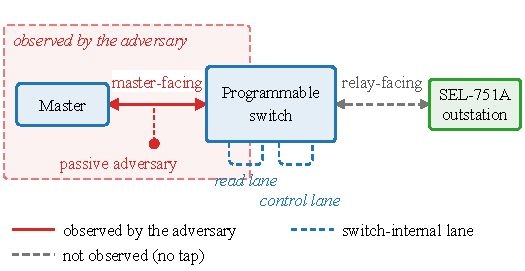
\includegraphics{figures/fig_observation}}{\figplaceholder{Observation model: master, observed master-facing link, programmable switch, relay-facing link (not observed), SEL-751A outstation.}}
\caption{Observation model. The adversary sees only the master-facing link (shaded); the relay-facing
  link and the switch-internal lanes (dashed) are observed by neither the adversary nor us.}
\label{fig:observation}
\end{figure}

\textbf{The adversary.} We assume a passive observer on the master-facing link, the adversary of
the fingerprinting attack we defend against~\cite{formbyWhosControlYour2016}.
Figure~\ref{fig:observation} shows where it sits. It records TCP and IP headers, segment sizes
and arrival times. It does not modify or inject packets, compromise the master or the outstation,
control the switch, or read the switch's internal state. It does not see the relay-facing link, which in our deployment is inside the switch with no tap
on it, and it does not see physical breaker motion.

Because DNP3 carries no transport security by default, we assume the traffic is
unencrypted~\cite{eastTaxonomyAttacksDNP32009}, so the observer also reads the DNP3 function
codes directly. An adversary that probes, injects, or otherwise acts on the network is out of scope. The
passive observer is the setting the traffic-obfuscation work we build on also targets.

\textbf{What the adversary is looking for.} Reconnaissance precedes the attacks that matter here. For example, false data injection
requires the attacker to know which devices it is dealing
with~\cite{liuFalseDataInjection2009}. Fingerprinting supplies that knowledge, and it does not
need the payload, because the timing of the exchange carries it. 

Following Formby et al.~\cite{formbyWhosControlYour2016}, two intervals are in scope. The first is
the CLRT of a READ or of the SELECT phase of a control, which measures the outstation's own
processing and which Section~\ref{sec:bg} shows carries the separation between the classes. The
second is the master-visible interval between an OPERATE's acknowledgment and its solicited
response. The adversary also sees the request-to-acknowledgment interval, whose median is 0.56~ms
on this device; the mechanism does not target it, and we report it as measured.

Our own observation is narrower than the adversary's in one direction and wider in none. Every
quantity we measure is one of three packet timestamps on the master-facing link: the request, the
acknowledgment and the response. The instants at which the switch releases a packet, and every
event on the relay-facing link, were not captured. Where the paper names them they come from the
configuration, and we say so.



The second interval deserves a careful statement, because it is easy to claim more for it than we
can support. Formby et al.\ estimate the time a device physically takes to complete an operation. However,
they do so from a sequence-of-events timestamp carried inside the outstation's application
payload, and their alternative estimate from packet arrival times produced no usable
result~\cite{formbyWhosControlYour2016}.  The interval we measure is a packet-timing feature of the solicited control response. It is not physical actuation time, and we do not measure physical actuation time anywhere. We
also make no claim about the payload-timestamp feature, which a mechanism that moves packets
without editing bytes could not affect in any case.

That narrower reading is still worth defending, because the interval separates the two classes on
its own and Section~\ref{sec:eval:ro3} shows an adversary recovering 0.651 balanced accuracy from
exactly that kind of difference. RO2 therefore asks whether the interval becomes a policy value,
not whether physical timing is concealed.

\textbf{What our evaluation actually separates.} Device fingerprinting is the application that
motivates the work. What we evaluate is narrower, and we keep the two apart throughout. Our
testbed has one outstation, so there is no second device to confuse it with and no device
identification to measure. What we measure is whether the timing of an exchange still reveals
\emph{which class of transaction} it was, on that one device. That is a three-class problem over
READ, SELECT and OPERATE, so chance is 0.333 balanced accuracy.  A result here is therefore the suppression of a class-conditioned timing feature, and not a
demonstration that two devices become indistinguishable.

\textbf{Two adversaries, not one.} We evaluate two conditions and report both. The \emph{fixed}
adversary learns transaction classes from undefended traffic and applies that model unchanged once
the defense is deployed; because the profile is built before the defense is met, this is the
adversary the reconnaissance setting describes. The \emph{adaptive} adversary collects obfuscated traffic and retrains on it, which answers what
remains learnable once the defense is deployed: it recovers 0.651 balanced accuracy where the
fixed one is left at chance. It needs no access the fixed one lacks, since the same passive
observer sees obfuscated traffic and the plaintext function codes label it; the two are evaluation
conditions rather than two adversaries with different powers. Both are ours, chosen to bracket the
problem, and the second is the one that limits our claim.

\textbf{Research objectives.} To make the goal checkable, we state it as five properties. The
evaluation answers each in turn, and we reuse the labels throughout.
\begin{itemize}
  \item \textbf{RO1 (read timing).} The visible CLRT of READ and of the SELECT phase of SBO is a
    configurable policy value rather than the outstation's own processing signature.
  \item \textbf{RO2 (control timing).} The master-visible OPERATE response-to-ACK interval stays at a
    policy value while the relay-facing hold is drawn from a configured codebook of 2, 6 and
    12~ms.
  \item \textbf{RO3 (timing leakage).} The timing features carry less information about the
    transaction class, and a fixed adversary that trained on undefended traffic is reduced to
    approximately three-class chance, which for READ, SELECT and OPERATE is 0.333 balanced
    accuracy.
  \item \textbf{RO4 (release policy and coverage).} The release budget, the range of policies the
    mechanism can realize, the fraction of traffic it can cover, and the residual it leaves are
    characterized rather than assumed.
  \item \textbf{RO5 (cost and protocol preservation).} We measure the latency the mechanism costs and the
    frames and bytes it adds, and the external DNP3 workload still completes: every request is
    answered and every control operation returns a success status.
\end{itemize}

\textbf{What is out of scope.} Two boundaries follow from the model above and hold for every
result we report. The framework does not hide the DNP3 function codes, which stay in plaintext, so
RO3 concerns the timing channel and not the command semantics. It also forwards every packet at
its original size, so it adds no size or segmentation signature of its own, while the delays it
imposes are themselves observable: an adversary who can time packets can see that something is
holding them. Because the relay-facing link is not instrumented, as stated above, the
per-transaction hold drawn from the configured codebook of 2, 6 and 12~ms is configured rather
than observed, which is why RO2 is stated in terms of the master-visible interval alone.

\section{Design}
\label{sec:design}

The objectives of Section~\ref{sec:threat} require a selected interval to become a value the
operator sets. We derive that from one transaction and defer the hardware realization to
Section~\ref{sec:impl}.

\subsection{A timing model for one transaction}
\label{sec:design:model}

\begin{figure}[t]
  \centering
  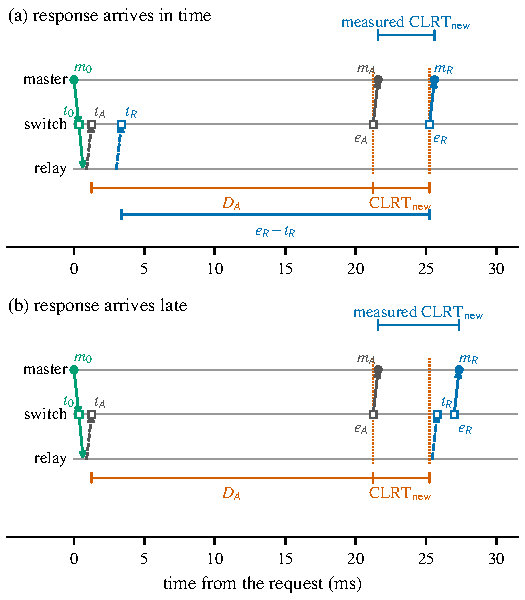
\includegraphics{figures/model/fig_m01_release_timeline}
  \caption{Release timeline of one READ transaction. Time coordinates are illustrative, chosen so
  an arrival and its emission are separable on the page. Both deadlines are computed from the
  acknowledgment's arrival $t_A$: in (a) the response arrives in time and the master observes the
  configured $\mathrm{CLRT}_{\mathrm{new}}$, in (b) it arrives late. The response hold $e_R-t_R$
  is drawn in (a) because the schedule implies it rather than configuring it. Filled circles lie
  on the master-facing link, the only place this work captured anything; open squares are
  switch-side instants that were not captured.}
  \label{fig:timeline}
\end{figure}

Consider one READ transaction, drawn in Figure~\ref{fig:timeline}. The master sends a request.
The outstation answers it twice: first its transport layer acknowledges the request, and later
its application layer returns the response with the data. We write $t_A$ for the instant the
acknowledgment reaches the switch and $t_R$ for the instant the response reaches it. The
switch forwards each packet onward at some later instant, $e_A$ and $e_R$ respectively. The
master therefore observes the interval $e_R - e_A$, up to the propagation and capture delay of
the two packets on the link between them.

That interval carries the information about the device, and on our relay it has a median of
2.116~ms for a poll and a spread of 2.6~ms:
\begin{equation}
\label{eq:clrt-original}
\mathrm{CLRT}_{\mathrm{original}} = t_R - t_A ,
\end{equation}
the time the outstation itself spends between acknowledging the request and producing the answer.
Section~\ref{sec:bg} explains why it identifies the device; here it is the quantity we intend to
remove.

To change what the master sees, the switch holds each packet. We write
\begin{equation}
\label{eq:holds}
D_A = e_A - t_A
\end{equation}
for the \emph{acknowledgment hold}, and we refer to $e_R - t_R$ as the \emph{response hold}
without giving it a symbol of its own, because the schedule below fixes it rather than letting us
choose it. Substituting into the interval the master observes gives the identity that governs the
whole design,
\begin{equation}
\label{eq:clrt-new}
\mathrm{CLRT}_{\mathrm{new}} = e_R - e_A
  = \mathrm{CLRT}_{\mathrm{original}} + (e_R - t_R) - D_A .
\end{equation}

Equation~(\ref{eq:clrt-new}) makes the difference between two kinds of defense concrete. If both
holds are constants, their difference is a constant and the observed interval is the original one
moved by it: the distribution slides along the axis and keeps its width, a spread of 2.6~ms
wherever it is moved to, so an observer who has seen the device before still recognizes it by the
shape. The response hold must instead absorb the variation in
$\mathrm{CLRT}_{\mathrm{original}}$, which we achieve by computing both releases from the same
instant $t_A$. When the acknowledgment arrives, the switch computes both release instants
immediately,
\begin{equation}
\label{eq:schedule}
e_A = t_A + D_A , \qquad e_R = t_A + D_A + \mathrm{CLRT}_{\mathrm{new}} ,
\end{equation}
where $\mathrm{CLRT}_{\mathrm{new}}$ is the interval we want the master to observe. These are the
\emph{scheduled} release instants. A packet's realized departure follows its scheduled instant by
the time the blocker queue takes to drain and by the queue's own service, which
Section~\ref{sec:impl} describes and Section~\ref{sec:eval:limits} measures on an instrumented
build, so the equalities here describe the schedule rather than the wire. We call this
value the \emph{configured} $\mathrm{CLRT}_{\mathrm{new}}$, and we call what the master actually
records the \emph{measured} $\mathrm{CLRT}_{\mathrm{new}}$; Section~\ref{sec:eval} reports how far
apart the two are. Because both release instants derive from $t_A$ and neither from $t_R$, the term
$\mathrm{CLRT}_{\mathrm{original}}$ cancels in~(\ref{eq:clrt-new}) and the observed interval is
the configured one. The response hold is therefore implied rather than chosen,
\begin{equation}
\label{eq:coupling}
e_R - t_R = D_A + \mathrm{CLRT}_{\mathrm{new}} - \mathrm{CLRT}_{\mathrm{original}} .
\end{equation}
Equation~(\ref{eq:coupling}) is why the three quantities cannot be picked independently: once the
acknowledgment hold and the configured $\mathrm{CLRT}_{\mathrm{new}}$ are fixed, the response hold
follows from whatever the device did on that transaction, and so varies from one transaction to
the next exactly as much as the device does.

This holds only while the response exists in time to be released on schedule. The switch can
delay a packet but cannot emit one it has not received, so~(\ref{eq:schedule}) requires
\begin{equation}
\label{eq:availability}
t_R \le t_A + D_A + \mathrm{CLRT}_{\mathrm{new}} .
\end{equation}
The acknowledgment may leave before the response arrives; that ordering is normal and does not by
itself imply a lost packet. When~(\ref{eq:availability}) fails the deadline is already past when
the response appears, so the switch marks it late and commits it to the response-hold queue, from
which it leaves when that queue next serves it, and the master observes an interval larger than
the configured value, as in Figure~\ref{fig:timeline}(b). One read-lane exchange in a thousand
answers too late to be scheduled. We report those rather than excluding them, because they are the
boundary of the mechanism and not a defect of the measurement.

The holds decide what the master observes \emph{between} the two packets, not how long it waits
for the answer itself, which is the quantity an operational requirement constrains. Write $D_R$
for that: the response's whole journey from the outstation transmitting it to the master receiving
it. We do not measure $D_R$, nor the portion of it from the switch onward, because only the
master-facing link is instrumented: $m_R$ is captured while $t_R$, the response's arrival at the
switch, is not. The quantity
\begin{equation}
\label{eq:resplatency}
m_R - t_R \le D_R
\end{equation}
is therefore a modelled partial journey, written from the model's endpoints rather than from
timestamps we hold, and full $D_R$ remains unmeasured.

Two terms make up the observed portion, $(e_R - t_R) + (m_R - e_R)$: the time the switch holds the
response and the path from the switch to the master. The hold itself divides once more, into the
wait to the release deadline, the interval $\varepsilon$ from that deadline to the end of
blocking, because the switch stops blocking a queued packet only once the queue gating it has
drained, and the service that follows. Those three sum to the hold rather than adding to it.
Consequently neither the response hold nor the configured $\mathrm{CLRT}_{\mathrm{new}}$ is the
response latency, and the three are not separately selectable: fixing $D_A$ and the configured
interval fixes the hold, which in turn consumes part of whatever the application deadline allows.
Section~\ref{sec:eval:limits} reports what we measured of $\varepsilon$ and on which build.

\subsection{Choosing the holds and the configured interval}
\label{sec:design:params}

The model leaves three quantities to decide: the acknowledgment hold $D_A$, the configured
$\mathrm{CLRT}_{\mathrm{new}}$, and, through~(\ref{eq:coupling}), the response hold that
follows from them. Each is limited by a different constraint.

The acknowledgment hold is limited in principle by the transport. Holding an acknowledgment delays the feedback the master's TCP uses to decide that a segment
is lost. Consequently, a hold approaching the master's retransmission timeout would make the
master resend a request the outstation had already answered.

That timeout has to be measured, not assumed.
RFC~6298~\cite{paxsonComputingTCPsRetransmission2011} recommends rounding it up to a second, but
that is a recommendation about a minimum and not a property every stack exhibits: on our master an
unacknowledged request is repeated after 201~ms. The 20~ms hold we evaluate consumes about a tenth
of that, and a hold of a few hundred milliseconds would begin to race it. We do not argue that the
timer's adaptivity makes a constant hold safe, because adaptation says nothing about the first
delayed exchange, a reconnection where the timer restarts, or a policy change mid-session.

In practice the transport bound is not the one that binds. The mechanism sustains a hold with a
budget on blocker passes rather than a wall clock, and from that budget, an assumed service rate,
a conservative bound on the outstation's acknowledgment latency, measured detection and release
terms and a safety margin, the control plane computes a horizon $H$ of 30.8~ms and an admissible
budget of 24.8~ms. Three limits act here and we keep them apart: the horizon is advisory and is
what the admission arithmetic reports; a separate clamp refuses any acknowledgment hold above
40~ms outright; and the sweep of Section~\ref{sec:eval:policy} deliberately installs settings past
the horizon to find where the mechanism leaves its operating region. None is a deadline the data
plane enforces, and the distinction matters because a pass budget bounds how many passes are
\emph{serviced}: under strict priority a lower-priority reservoir can be starved while a
higher-priority one is still being served, so one budget does not translate into one elapsed time
for every queue. The sweep of Section~\ref{sec:eval:policy} shows the consequence directly:
at a configured acknowledgment hold of 36~ms the median request-to-acknowledgment interval
saturates at 31.07~ms, well short of the configured value, while the median request-to-response
interval for the same point is 40.58~ms and the median CLRT is 9.51~ms rather than the
configured 4~ms. The acknowledgment reaches a ceiling; the response does not stop at it. That
saturation is an observed transition for the acknowledgment lane at this configuration, not a
release deadline the hardware guarantees for every held packet.

The configured $\mathrm{CLRT}_{\mathrm{new}}$ is limited by the operation, and through $D_R$
rather than directly: what an operator can accept is a bound on how long the answer takes to
arrive, not on the gap between the two packets that carry it. We could not verify a communications
requirement that fixes such a bound for a DNP3 poll or a select-before-operate control on a
distribution relay. The only numeric deadline we could verify from primary documentation is the
relay's own select-to-operate timeout, documented default
1.0~s~\cite{selSEL751AInstructionManual}, which governs how long a select stays armed rather than
how quickly a response must return, and timing classes defined for other protocols do not transfer
to a DNP3 poll merely because their numbers are convenient.

We therefore treat the setting as a deployment choice rather than a compliance question, state the
value we tested, 4~ms, and report the response latency the mechanism produces, about 23~ms more
than the device alone, so an operator with a requirement of their own can check it against those
numbers.

Together the two set what the mechanism costs. Their sum
\begin{equation}
\label{eq:budget}
D = D_A + \mathrm{CLRT}_{\mathrm{new}}
\end{equation}
is the release budget: by~(\ref{eq:availability}) it decides which transactions the switch can
place on the schedule at all. A larger budget covers more of the device's own response-time
distribution and costs more delay on every transaction it covers: at $D=24$~ms it covers 99.9\% of
them for about 23~ms of added latency. $D$ is the budget and not the delay added to each exchange,
since a transaction the outstation answers quickly is held longer than one it answers slowly, so
the added delay is at most $D$ rather than equal to it.

Because the budget and the observable are different quantities, an operator can fix the cost and
still choose the feature: holding $D$ at 24~ms, we installed configured values from 1~ms to 22~ms
and the master observed each one while the added delay stayed the same.
Section~\ref{sec:eval:policy} reports that sweep and the point at which the realized hold stops
tracking the requested one.

The model says nothing about what $\mathrm{CLRT}_{\mathrm{new}}$ should be, so the framework and
the policy it carries are separate. We chose a constant, because it removes the device's variation
entirely and is the simplest policy to state and to check. A schedule could instead draw the value
from a distribution or make it a function of the operation, and the same mechanism would carry it;
we implement and evaluate only the constant setting.

\subsection{The control transaction is timed from the request}
\label{sec:design:control}

A select-before-operate control command differs in one way that matters here: the framework holds
the command itself before it reaches the relay, separating the moment the master issued the
command from the moment the relay acts on it. The outstation's acknowledgment cannot be the
reference instant, because it does not exist until after the command has been released, and any
deadline measured from it would carry the length of the command hold into the interval the master
observes. We therefore time the control lane from the request. When
the OPERATE arrives at $T_0$, the switch releases it toward the relay after an internal
delay $J$. It places the acknowledgment and the solicited response the master sees at configured
offsets from $T_0$,
\begin{equation}
\label{eq:control}
e_{\mathrm{ack}} = T_0 + A , \qquad e_{\mathrm{or}} = T_0 + R .
\end{equation}
Consequently, the interval the master observes is
\begin{equation}
\label{eq:optime}
O = e_{\mathrm{or}} - e_{\mathrm{ack}} = R - A ,
\end{equation}
in which $J$ does not appear, so the relay-facing release time can vary while the master-facing
interval does not, and an observer cannot subtract a known offset to recover it.

The control plane checks that $A$ exceeds the largest admissible $J$ plus the outstation's own
acknowledgment latency before it installs the values, since a deadline the switch cannot honor
would fail open rather than protect. In our experiments $D_A$ is 20~ms, $\mathrm{CLRT}_{\mathrm{new}}$ is 4~ms, and $R - A$ is
also 4~ms, so the two lanes present the same value to the observer.

\subsection{What the design does not change}
\label{sec:design:boundary}

The mechanism replaces one interval per lane and leaves the rest of the exchange as it was. The
DNP3 function codes remain in plaintext and every packet's direction remains visible, so an
observer can still tell a poll from a control command by reading the packet, and the
request-to-acknowledgment interval still contains the outstation's own acknowledgment latency,
displaced by the constant $D_A$ but not reshaped by it. The switch forwards the packets it
received without padding them, injecting new ones or editing any DNP3 field, which is what the
plaintext setting requires and which leaves every size feature as it was. It does change when
packets leave, so it is not a claim about arrival order.
Section~\ref{sec:eval:ro3} reports what an attacker allowed to retrain on the obfuscated traffic
still recovers from the features that remain.

\section{Implementation}
\label{sec:impl}

Section~\ref{sec:design} says when each packet should leave, but a forwarding pipeline has no way
to wait: a P4 program runs to completion per packet and can read a clock, yet it cannot sleep or
schedule a callback.

\subsection{Holding a packet with queues}
\label{sec:impl:queues}

\begin{figure}[t]
\centering
\IfFileExists{figures/fig_design.pdf}{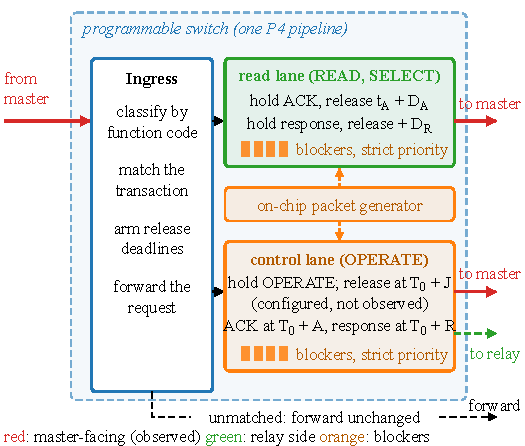
\includegraphics{figures/fig_design}}{\figplaceholder{One P4 pipeline: ingress classifies and arms deadlines; a read lane holds the acknowledgment and the response; a control lane holds the OPERATE; blocker reservoirs drained by a strict-priority scheduler realize the deadlines; unmatched traffic is forwarded.}}
\caption{How one pipeline realizes the schedule. Ingress classifies each transaction and computes
  its release deadlines. Blocker packets drained ahead of the held packet sustain a hold until its
  deadline expires. The four-queue ladder holds what the outstation returns; the second pair holds
  the outgoing OPERATE, not a second reply. Solid lines are master-facing and observed; dashed
  lines are not, as in Figure~\ref{fig:observation}.}
\label{fig:design}
\end{figure}

What the switch does have is a traffic manager with several queues per port and a strict-priority
scheduler, the primitive with which SP-PIFO approximates programmable scheduling on today's
hardware~\cite{alcozSPPIFOApproximatingPushIn2020}. A scheduler decides what does \emph{not}
leave, and we hold a packet by using that property rather than a timer.

A READ uses \emph{four} queues on one internal port, as Figure~\ref{fig:design} shows. Two carry
the packets we delay, the acknowledgment and the response, and above each of those sits a
\emph{blocker queue} in strict priority carrying small packets the switch generates itself. While
blockers keep arriving, the packet beneath them is never served, and each hold ends when its own
blocker queue runs dry. The response is not simply queued behind the acknowledgment: it has its
own held queue and its own blocker gate, which is what lets the two releases be scheduled
independently. In descending priority the ladder is acknowledgment blockers, held
acknowledgment, response blockers, held response.  Blockers circulate on an internal loopback port and never reach a cable, so neither endpoint
can observe them. Each carries a tag naming its transaction and lane, so a leftover blocker
cannot delay a later transaction.

This is not a timer built from a count. The program stores an absolute release instant when the
acknowledgment arrives, quantized to a 256~ns grid, and each of the 64 recirculating blockers
compares the current timestamp against it: while the difference is negative the blocker is
regenerated, and once it is not, the blocker is dropped. The deadline decides when the packet
leaves, and the blockers only have to keep the queue non-empty until then, so the reservoir is
sized for continuity rather than for duration.

The queue does not empty at the deadline, however. Each blocker tests the deadline on its own
pass, so those still queued when it passes are served once more before the queue runs dry and the
held packet leaves. The release therefore trails the deadline by the time that draining takes, and
each lane drains its own queue, the acknowledgment's above the response's;
Section~\ref{sec:eval:limits} reports what we measured of that interval. The arrangement is what
makes the coupling of Section~\ref{sec:design:model} implementable: the response's release instant
is computed at the acknowledgment, so the hold absorbs whatever the outstation does without the switch measuring it.

\subsection{One READ transaction}
\label{sec:impl:walkthrough}

The request arrives, a table classifies it by function code, and the program forwards it at once,
recording that a transaction is in flight and which acknowledgment to expect. When the
acknowledgment arrives at $t_A$, a median of 0.56~ms after the request on our relay, the
program writes both release instants from that one timestamp, which is what puts them on the
same instant $t_A$ that Section~\ref{sec:design:model} requires. It does so once from an unarmed sentinel so a duplicate acknowledgment cannot arm a
second deadline. The acknowledgment enters the hold queue and the packet generator fills the
blocker queue. A response that arrives before its deadline queues behind the acknowledgment,
and the two leave in order at their scheduled instants. A response that arrives after its deadline has no remaining wait to serve, and the program marks
it late and commits it to the same response-hold queue rather than to a bypass, as in
Figure~\ref{fig:timeline}(b); it leaves when that queue next serves it, so its departure is
prompt but not instantaneous. The transaction state is cleared when the response is released.

The two lanes hold different packets, and it is worth saying which. The four-queue ladder above
holds what the outstation sends back, the acknowledgment and the response, for READ and for both
phases of a control alike. The second loopback port carries a pair of queues for the opposite
direction: blockers above a held \emph{OPERATE request}, on its way to the relay. So the control
extension adds a hold the read path does not have, while the packets the master observes are
released by the same machinery in both cases. Giving the OPERATE its own scheduling domain keeps
it from being starved by the higher-priority read reservoirs.

The queues are separate; the transaction state is not. The deadline registers are shared. Every register that
records a transaction holds a single slot, and the control path writes the same release instants
at OPERATE admission that the read path uses, so the program protects one transaction at a time
rather than one per flow.

The evaluated configuration satisfies that assumption by construction: the driver serialises its
exchanges and every capture carries one connection. Where a second transaction would arm while one
is live, the program does not interleave them silently; the arming attempt is classified as busy
and the packet is forwarded unprotected rather than taking the deadline already in progress. That
is a statement about the deadline, not about the rest of the transaction's state: the expected
relay sequence and acknowledgment are written earlier in the same pass than the busy verdict is
reached, so we claim it for the serialized workload we evaluated and not in general. Per-flow
protection would need per-flow state and a way to index it, which this program does not have and
we did not evaluate.

\subsection{Failing open}
\label{sec:impl:failopen}

Almost every path through the program ends in a forwarding decision. A packet outside the protected
session, an unrecognized request, an acknowledgment with no armed transaction and a response whose
transaction has retired are all forwarded unchanged, so such an exchange loses its protection and
still arrives. One path is not like that, and we state it here rather than in the evaluation: the
control lane keeps a released OPERATE's application generation as a spent marker until the next
SELECT clears it, and a later OPERATE carrying that generation is dropped. A retransmission the
master sends to repair an OPERATE lost after the switch forwarded it carries exactly that
generation, so the switch discards the packet that would have repaired the loss
(Section~\ref{sec:eval:limits}). Every hold is bounded by a budget on blocker passes: once a reservoir has spent
its budget the packet is released and its state cleared. That budget counts passes rather than
elapsed time, which is why the horizon $H$ of Section~\ref{sec:design:params}, 30.8~ms here, is
what the control plane computes from the budget and an assumed service rate rather than a
wall-clock deadline the data plane keeps. With the timing mode off the same program forwards
everything immediately, which is how we collected the Timing OFF arm.

\subsection{Resources and testbed}
\label{sec:impl:p4}

The program is about 1{,}560 lines of
P4$_{16}$~\cite{bosshartP4ProgrammingProtocolIndependent2014} for the Tofino Native
Architecture, compiled
with the Barefoot SDE 9.13. It occupies all twelve ingress match-action stages of one pipeline and six egress stages, with
112 tables. State is small: one-entry registers reached by stateful ALU actions, one access per packet per
register, which is what the architecture permits. One 25~Gb/s port carries the master and one 1~Gb/s port the relay, and two further ports are
loopbacks carrying no cable: the first carries the four-queue read ladder, the second the control
extension's pair, blockers above a held OPERATE, in its own scheduling domain so the OPERATE
reservoir cannot be starved by the higher-priority read reservoirs. Six queues across two
loopbacks in all.

Every policy quantity is a runtime table entry, so an operator changes policy by writing entries
rather than loading a program. The loaded build realizes the dual-deadline schedule only: its
arming table admits that mode alone, so the acknowledgment-only and response-only limits of the
model are properties of the design and not settings of this build, and configuring them left both
packets unheld with the measured interval the outstation's own.

The control plane, about 890 lines of Python, brings up ports and queues, installs the
packet-generator configuration, and writes the timing parameters and reads them back. What it
refuses is a clamp, not the admission arithmetic: a request for an acknowledgment hold above
40~ms is rejected outright before any write, which we confirmed on the switch, and the
acknowledgment offset $A$ on the control lane must exceed the largest admissible $J$ plus a bound
on the outstation's acknowledgment latency. The horizon $H$ of
Section~\ref{sec:design:params} is computed and reported, not enforced, which is exactly why the
sweep of Section~\ref{sec:eval:policy} can install settings beyond it and find where the
mechanism leaves its operating region. The outstation is an SEL-751A feeder
protection relay, one of the DNP3 device classes whose timing Formby et al.\
fingerprint~\cite{formbyWhosControlYour2016}. The master issues READ and select-before-operate
operations to isolated control points through a guarded driver, so no control operation in the
evaluation moves a breaker.

\section{Evaluation}
\label{sec:eval}

\subsection{What we measured, and where}
\label{sec:eval:testbed}

\textbf{Evaluation Cases.} We compare two arms of the same program, differing only in the release
schedule. In \emph{Timing OFF} the switch forwards the outstation's acknowledgment and response as
they arrive; in \emph{Obfuscated} it holds them and releases them on the deadlines of
Section~\ref{sec:design}. The switch is the only path between the master and the relay, and every
timestamp is taken on the master-facing link, so each interval below is one a passive observer can
record: the arrival of the transport acknowledgment to the arrival of the application response,
both on the master's own interface. The switch's internal instants are on links that were not
captured and are recovered from the program rather than measured.

\textbf{Configuration provenance is partial.} Each block's manifest records the policy it was
configured with and the loaded program's identity, but the sweep has no per-point readback of what
the device held. Every policy value in this section is the configured one unless we say otherwise,
and we mark where a readback would have settled a question the configuration cannot.

\textbf{Dataset.} We report per DNP3 exchange. The campaign holds 63{,}360 of them, half with the
mechanism running and half without, collected over five hours in interleaved blocks so that drift
cannot separate the two arms. Every request was answered, and no exchange was retransmitted,
malformed or excluded. A separate sweep on the same testbed covers 16 configured policies and
three controls with the mechanism disabled.

\subsection{Does the released interval reach its configured value? (RO1)}
\label{sec:eval:ro1}

\begin{figure}[tbp]
  \centering
  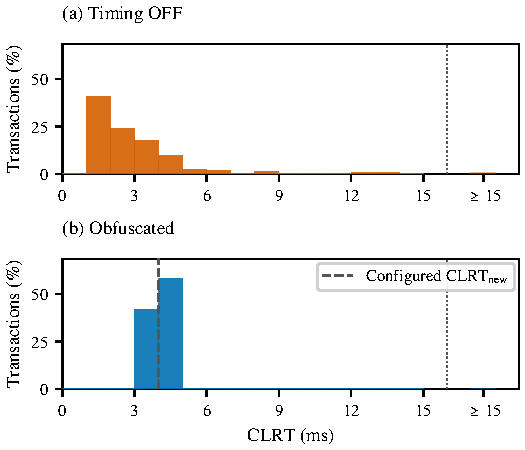
\includegraphics{figures/clrt/fig_clrt_distributions}
  \caption{Measured READ CLRT before and after obfuscation, as the percentage of each arm's own
  transactions per bin, on common 1~ms bins anchored at 0~ms with a linear ordinate. Finite bins
  are half-open; the hatched category holds everything at or above 15~ms, 0.409\% of (a) and
  0.027\% of (b). The dashed line in (b) is the configured $\mathrm{CLRT}_{\mathrm{new}}$, which
  falls on a bin edge, so the obfuscated mass divides between the two neighbouring bins;
  Figure~\ref{fig:clrtzoom} resolves it. In (a) $n$~=~26{,}400, mean 2.800~ms, sd 2.609~ms,
  variance 6.808~ms$^2$; in (b) $n$~=~26{,}400, mean 4.012~ms, sd 0.628~ms, variance
  0.394~ms$^2$.}
  \label{fig:hist}
\end{figure}

\begin{figure}[tbp]
  \centering
  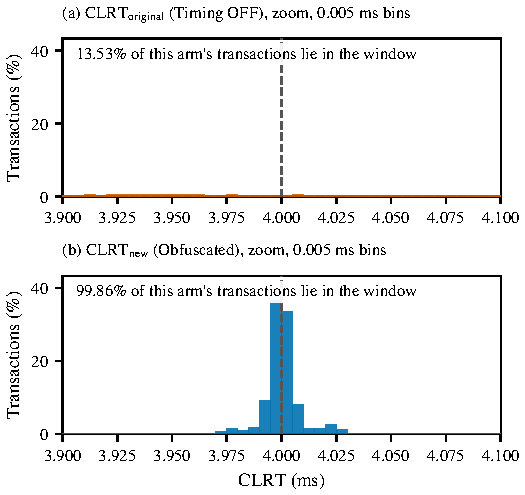
\includegraphics{figures/clrt/fig_clrt_zoom}
  \caption{The released interval, resolved. The same measurements as Figure~\ref{fig:hist} on
  0.005~ms bins within $0.10$~ms of the configured $\mathrm{CLRT}_{\mathrm{new}}$ (dashed). The
  ordinate is still the percentage of that arm's entire sample, not of the window, so the bars
  are directly comparable with the other figures. The window holds 13.58\% of (a) and 99.86\% of
  (b).}
  \label{fig:clrtzoom}
\end{figure}

\textbf{RO1.} The read-path schedule of~(\ref{eq:schedule}) does replace
$\mathrm{CLRT}_{\mathrm{original}}$ with the configured $\mathrm{CLRT}_{\mathrm{new}}$. We compare
the two arms over all 22 grouped runs as full empirical distributions, because the shape of the
Timing OFF distribution is what makes a single observation informative to an adversary.

Figure~\ref{fig:hist} shows the two READ distributions. Before obfuscation the interval is broad
and multi-modal, spanning 1.01 to 83.46~ms with peaks near 1.2, 2.1 and 4.0~ms; after it, 99.9\% of
transactions fall within 0.10~ms of the configured $\mathrm{CLRT}_{\mathrm{new}}$. In
Figure~\ref{fig:clrtzoom} the released interval resolves into a narrow distribution about that
value, where the Timing OFF arm places only 13.6\% of its transactions.

The change is a replacement, not a shift. The standard deviation falls from 2.609 to 0.628~ms for
READ and from 2.267 to 0.024~ms for SELECT, variance ratios of 0.058 (95\% CI [0.019, 0.101]) and
0.0001 (95\% CI [1.4$\times$10$^{-5}$, 3.4$\times$10$^{-4}$]) under a session-level bootstrap. A
defense that shifted the interval would keep that spread, because translating a sample leaves its
variance unchanged: translated onto the protected median, the Timing OFF distribution retains
standard deviations of 2.609 and 2.267~ms, four and ninety-four times what we measure. That
counterfactual is analytical, computed from the Timing OFF samples themselves; the loaded program
has no shifting mode, so it is not a measured arm and we do not present it as one.

Low spread at the wrong interval would not be normalization, so we also report where it sits.
The median $\mathrm{CLRT}_{\mathrm{original}}$ is
2.116~ms for READ and 2.050~ms for SELECT, with interquartile ranges of 2.778 and 2.697~ms; under
the mechanism both medians are the configured 4.000~ms and each interquartile range falls to
0.006~ms, two orders of magnitude below the 1~ms step between neighbouring policy settings in the
sweep of Section~\ref{sec:eval:policy}. The median alone understates the change, because the
Timing OFF distributions rise in a few discrete steps, so one observation can be informative about
the class, whereas the obfuscated ones are a step at the scheduled release, an instant computed
from the acknowledgment and a fixed offset that no longer depends on how long the device took.
Figure~\ref{fig:hist} shows that for READ; the per-class distributions for all three, and the
per-run medians in acquisition order, are published with the artifact.

A tail remains, and it is one-sided: the largest obfuscated READ interval is 57.182~ms, and fewer
than one READ exchange in a thousand departs from the scheduled release by more than 1~ms. The
asymmetry follows from the mechanism, because a response reaching the switch after its scheduled
release cannot be moved backwards and leaves as soon as the hold queue serves it. The mechanism
cannot schedule a release before the response exists. Below the configured value the distribution
is not empty either: each release carries its own queueing and service, so their difference falls
either side of the configured interval, which is why the distribution has width at all. Those late
exchanges are the coverage boundary of RO4 seen from the other side, and we count them rather than
hide them.

\textbf{Stability within the Campaign.} The obfuscated median sits at the scheduled release in
every one of the 22 grouped runs and every class, while the Timing OFF medians stay separated, so
the effect is not an artifact of one run or of drift over the five hours. The per-run medians and
interquartile ranges in acquisition order are published with the artifact.

\subsection{Does the control lane behave the same way? (RO2)}
\label{sec:eval:ro2}

\textbf{RO2.} The control-path rule of~(\ref{eq:control}) holds the master-visible
response-to-ACK interval at the policy value. Timed from the request, its observable is
$O = R - A$, in which the internal hold $J$ does not appear, so the read-path budget $D$ does not
apply to it; the switch draws $J$ per transaction from the configured codebook
$\{2, 6, 12\}$~ms. The OPERATE median moves from 2.937~ms under
Timing OFF to 4.000~ms under the mechanism, the interquartile range falls from 2.827 to 0.006~ms,
and the interval stays concentrated at the configured value in every run. That is a result about
the interval the master sees: the relay-facing release at $T_0 + J$ was not observed
(Section~\ref{sec:eval:limits}).

\subsection{What range of settings does the mechanism support? (RO4)}
\label{sec:eval:policy}

\begin{figure}[tbp]
  \centering
  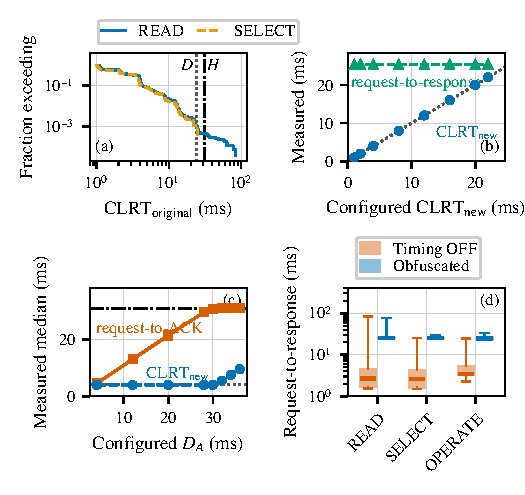
\includegraphics{figures/ndss/fig_policy_coverage_cost}
  \caption{The release policy is programmable and bounded on both sides. (a) Timing OFF read-lane tail
  against the budget $D$ and the horizon $H$. (b) At $D=24$~ms the measured $\mathrm{CLRT}_{\mathrm{new}}$ follows the
  configured $\mathrm{CLRT}_{\mathrm{new}}$ while the response latency stays fixed. (c) Raising $D_A$ saturates near $H$.
  (d) End-to-end response time per class.}
  \label{fig:policy}
\end{figure}

\textbf{RO4.} The interval a passive observer records is a policy value the operator sets, over a
usable range. We installed 16 release policies in turn and ran a fixed DNP3 workload through each,
in two series: the first holds the budget at $D = D_A + \mathrm{CLRT}_{\mathrm{new}} = 24$~ms and
moves the split between them, the second fixes the configured
$\mathrm{CLRT}_{\mathrm{new}}$ at 4~ms and raises $D_A$ until the mechanism leaves its operating
region. Each point is the median over its READ exchanges.

In Figure~\ref{fig:policy}(b) the measured $\mathrm{CLRT}_{\mathrm{new}}$ follows the configured
value along the identity line: settings of 1, 2, 4, 8, 12, 16, 20 and 22~ms give measured medians
of 0.998, 1.999, 3.999, 8.001, 12.001, 16.000, 20.001 and 22.001~ms, while the end-to-end response
time stays between 25.30 and 25.34~ms throughout. The leaking interval and the cost of the
exchange can therefore be set independently, which is what makes the mechanism a framework rather
than one fixed setting. In Figure~\ref{fig:policy}(c) the request-to-acknowledgment interval
tracks $D_A$ up to 30~ms, where the measured median is 30.571~ms and
$\mathrm{CLRT}_{\mathrm{new}}$ still sits at 4.001~ms.

Beyond that the acknowledgment interval saturates at about 31.07~ms and
$\mathrm{CLRT}_{\mathrm{new}}$ can no longer be held, rising to 5.503, 7.498 and 9.507~ms at $D_A$
of 32, 34 and 36~ms, because the reservoir carries a finite pass budget and a hold ends when that
budget is spent. The saturation sits close to the admission horizon $H$, which is what one would
expect if the control plane's assumed service rate is about right, but is not evidence that the
data plane enforces $H$. From below the range is closed by the outstation's own response time,
which the switch cannot anticipate: in Figure~\ref{fig:policy}(a) the 24~ms budget covers
99.900\% of Timing OFF read-lane exchanges, and one in a thousand arrives too late to be held. The
usable range is therefore 1 to 22~ms at a fixed budget.

\subsection{What does the mechanism cost? (RO5)}
\label{sec:eval:cost}

\textbf{RO5.} In Figure~\ref{fig:policy}(d) the median response time rises by 22.7~ms for READ,
22.6~ms for SELECT and 21.2~ms for OPERATE: close to but below the release budget, because it
depends on how long the outstation itself took, and a real operational cost to weigh against the
polling period and any protocol timeout. Each exchange carries 3.017 frames and 272.3 bytes on the
master-facing link, identical in both arms, so the mechanism moves packets in time without adding
a frame or a byte.

\textbf{Timeout and Retransmission Headroom.} Holding the acknowledgment consumes the master's
timers, so we measured what it consumed. On the master-facing captures the request bytes were
acknowledged in a separate segment every time, never piggybacked on the response, no request was
sent while earlier bytes were unacknowledged, and there was no retransmission, reset or duplicate acknowledgment in either arm.

The longest the master waited for its acknowledgment was 29.2~ms and for its response 77.7~ms.
Withholding every acknowledgment of one request on a separate diagnostic connection, we observed
the master repeat it after 201~ms, about seven times the longest observed wait, which is
consistent with the absence of a retransmission. The 201~ms is a measured repetition threshold
rather than a reading of the sender's timer: the capture records packets, not socket state, and
the next repeat followed 208~ms later, which simple exponential backoff does not explain. The
receive timeout in our driver is 3~s and bounds one read rather than the whole transaction, so it
is not a transaction deadline.

Select validity is the other timer a held control transaction could violate, since the master
issues its OPERATE only 0.19~ms after the SELECT response reaches it and the mechanism delays that
response: no obfuscated OPERATE exchange was refused for a stale select. All of this characterizes
this operating point, and would have to be rechecked for a master with a shorter timeout.

\subsection{What does the attacker still learn? (RO3)}
\label{sec:eval:ro3}

\begin{figure}[tbp]
  \centering
  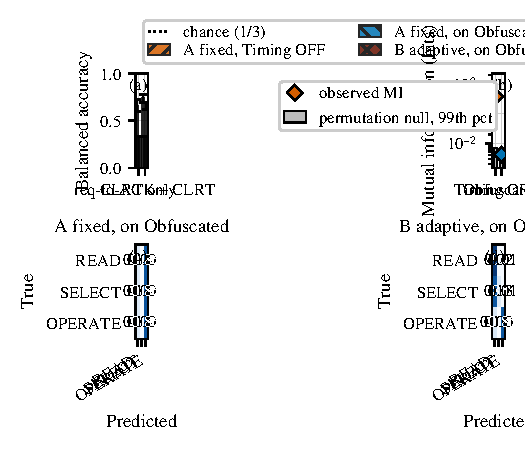
\includegraphics{figures/ndss/fig_leakage}
  \caption{Transaction-class leakage under the two attacker models, leaving out one grouped run at a time.
  (a) Balanced accuracy; whiskers span the 22 held-out runs and are not a confidence interval.
  (b) Mutual information against a within-run permutation null. (c) and (d) Row-normalized
  confusion using both intervals.}
  \label{fig:leakage}
\end{figure}

\textbf{Setup.} The features are the two separately measurable intervals; their sum, the total
response time, is excluded so that no feature is a linear combination of the others. Separately
measurable is not statistically independent and we do not assume it is: the classifier is given
both and may exploit any dependence between them, which is what the adaptive result below does. We
estimate mutual information for the CLRT in bits against a null built by shuffling class labels
within each grouped run over 1{,}000 permutations, preserving the per-run class counts. Every fold
leaves out one grouped run, and we report the spread of the 22 held-out-run scores as a range.

\textbf{RO3.} Consider first what the mechanism does to the two intervals before any classifier is
applied. Under Timing OFF the classes separate mainly along the post-acknowledgment axis, with
medians of 2.116, 2.050 and 2.937~ms for READ, SELECT and OPERATE against
request-to-acknowledgment medians of 0.555, 0.555 and 0.558~ms, which barely separate them at all.
Under the mechanism that axis collapses: all three medians sit at 4.000~ms and READ and SELECT
overlap. What remains is a horizontal offset, with the request-to-acknowledgment median moving to
21.336, 21.239 and 20.650~ms, because the read lane is timed from the outstation's acknowledgment
and the control lane from the request. The two intervals plotted against each other, which is how
that collapse and that offset look, are published with the artifact.

In Figure~\ref{fig:leakage}, we show the two attacker models.

The fixed adversary trained on
Timing OFF traffic reaches 0.652 balanced accuracy on held-out Timing OFF exchanges using the
CLRT alone, and 0.736 using both intervals. Applied unchanged to obfuscated traffic, it falls to
0.333 and 0.334, which is chance. Mutual information between the CLRT and the class falls from
0.383~bits to 0.004~bits; the Timing OFF value lies far above its permutation null at the
resolution of the test ($p = 0.001$ with 1{,}000 permutations), and the obfuscated value lies
inside its null ($p = 0.084$), so the test does not reject the hypothesis that the obfuscated
estimate is null noise. Failing to reject is not evidence of zero: with 1{,}000 permutations the
test resolves differences of this size only so far, and a small residual dependence would look the
same. For the evaluated fixed Random-Forest attacker, then, three-class transaction identification
falls to approximately chance, and no dependence between the cross-layer response time and the
class survives at the resolution of this test. Note that this holds for the two features we give it; the plaintext function code is
outside a timing-only feature set and still names the operation. 

The adaptive adversary gives two results, and they answer different questions. Retrained on
obfuscated traffic it stays at chance, 0.333, on the CLRT alone: the targeted feature is
suppressed against a retrained adversary and not only against a fixed one. The same adversary
recovers to 0.651 when it is given both intervals, because the read and control paths are timed
from different events, so their acknowledgment latencies differ. The confusion panels show the
shape of that recovery, with OPERATE separable while SELECT stays confused with READ.

We state the cost of that difference rather than leave it to be inferred. On the
request-to-acknowledgment interval alone, balanced accuracy rises from 0.380 under Timing OFF to
0.662 under the mechanism: almost nothing about the class before the mechanism runs, and the most
informative single feature afterwards. The mechanism does not merely fail to remove that feature,
it creates it, because holding the acknowledgment for $D_A$ displaces an interval the two lanes
compute from different events. Against an adversary using both intervals and allowed to retrain,
the net effect is a fall from 0.736 to 0.651, or 0.085 on a three-class problem whose chance is
0.333.

The targeted feature is therefore suppressed under both conditions, the cross-layer response time
alone leaving fixed and retrained adversaries alike at 0.333. What retraining recovers, it
recovers from the request-to-acknowledgment interval, which the mechanism does not target and does
make more informative, and that residual bounds the result. Formby et
al.~\cite{formbyWhosControlYour2016} profile devices from undefended traffic, which motivates the
fixed condition; their setting does not restrict an observer of this mechanism to an unchanged
model, and we do not read it as doing so. One way to close the residual is to time both paths
from the same event, which we leave to future work. We do not claim it is the only way: we have
not searched the space of defenses that might close it differently.

\subsection{Limitations}
\label{sec:eval:limits}

Each limitation below bounds one of the results above, and we name which.

\textbf{One Device, One Campaign.} The evidence is one SEL-751A behind one Tofino-1 in one
five-hour campaign, and the runs are grouped collections rather than independent replications, so
every result from RO1 to RO5 is a statement about this device and this window and every spread is
within-campaign variability.

\textbf{What RO3 Establishes.} RO3 characterizes the Random-Forest attacker we evaluated rather
than every classifier, and the adaptive adversary recovers 0.651 balanced accuracy from the
difference between the two events, which is the bound on what it achieves.

\textbf{What RO2 Rests On.} Only the master-facing link was captured, so the realized
per-transaction hold $J$ and the relay-facing release at $T_0 + J$ are configured rather than
observed: RO2 is a claim about the interval the master sees and reports no result per $J$.

\textbf{What RO4 Observes.} The admission horizon $H$ is computed in the control plane rather than
enforced by the data plane, so the saturation at 31.07~ms is an observed transition and not a proof
that the two coincide, and the sweep offsets likewise come from the configuration table rather
than a per-point readback.

\textbf{The Residual Is Not Attributed.} The switch's own release instants were not captured, and
the program cannot supply them: the timestamp registers it declares are never written. What the
measured distribution shows around the configured value is therefore a net difference between two
releases, not a delay we can place inside the switch.

On a separately instrumented build that adds two registers per lane, keyed on the outcome marking
a blocker that terminates because its deadline passed, the medians over twelve transactions are
1{,}706~ns on the acknowledgment lane and 1{,}705~ns on the response lane, with standard
deviations of 8.7 and 8.0~ns, about $4\times10^{-4}$ of the 4~ms configured interval. The first
blocker's ingress timestamp follows the deadline by a median of 12.5 and 13.5~ns, bounding when a
blocker first observed the expiry rather than when the release decision was taken, which the
program does not timestamp.

Four limits apply, and the first is why we do not simply call it $\varepsilon$. Both timestamps
are taken in ingress on a recirculating blocker token, so the interval ends at the last blocking
action and not at the wire, and this program carries no egress timestamp. We report an internal
blocker-termination interval and do not claim it bounds $\varepsilon$ in either direction, because
the blocker's last traffic-manager service precedes its return to ingress and the ordering of the
two endpoints is not established. It comes from a \emph{different build} than the campaign, so it
characterizes the mechanism rather than any exchange in the measured distributions; that build is
identified by the recorded patch over the frozen program, with the build tree, its loader
configuration and the loader's log agreeing on which binary ran. Twelve transactions at one
configuration are not a drain bound over load. Comparing the instrumented build against the frozen
one over 200 polls each gives mean cross-layer response times of 4.000282 and 3.999470~ms with
sample standard deviations of 0.0153~ms in each: one pair of captures at one configuration, which
does not establish equivalence, and which would not reveal equal movement in both releases.

\textbf{What RO5 Counts.} The overhead of RO5 is measured on the master-facing link, where the
switch's internal blocker traffic never appears. The zero-retransmission result is bounded the
same way: because the program suppresses a response retransmission that matches an already-seen
transport position while its transaction is live, such a copy would be absorbed inside the switch
and would not reach a master-facing capture.

We probed that suppression. A response lost downstream of the switch is recovered by exactly such
a retransmission, so a mechanism that discarded it would break loss recovery. Dropping the
response inbound at the master, scoped to one connection, leaves it unacknowledged and the
outstation retransmits on its own timer; three further copies crossed the switch and reached the
master's interface, at 3.20, 9.21 and 20.25~s, every one forwarded rather than absorbed.

The probe does not show that duplicate suppression preserves loss recovery. The filter dropped
every copy for the whole test rather than only the original, so nothing was acknowledged and the
application recovered nothing, and the capture is taken ahead of the filter, so it records arrival
at the interface. The copies also arrived long after the transaction had retired, the first
2.97~s after a transaction live for about 24~ms, so they met the path a stale token takes rather
than the path a duplicate of a live transaction takes, which is the case the concern is about.
Reaching that path needs an outstation whose retransmission timer is of the same order as the
hold; on this relay it is about three orders larger. The mechanism forwards late copies, and the
live-window case stays open.

\textbf{A Lost OPERATE Cannot Be Repaired.} The control lane has a second and worse case, which we
found by reading the program rather than by measuring it. After the switch releases an OPERATE
toward the relay it keeps that command's application generation as a spent marker, and clears it
only when the next SELECT arrives. A later OPERATE carrying the same generation is classified a
duplicate and dropped. If the released command is lost on the relay-facing link, the master's
transport repairs the loss by retransmitting exactly those bytes, with the same generation, and
the switch discards the packet the repair depends on. Forwarding a command out of the switch is
not delivery to the relay, and the program cannot tell the two apart because the relay-facing link
is not instrumented. No capture in this work exercises the path: the campaign's 5{,}280 OPERATE
exchanges lost nothing and every control operation returned success, which is the normal case
working rather than evidence that the failure case is handled. We therefore claim no loss recovery
on the control path, and exactly-once execution is neither provided nor claimed.

\textbf{The Tail Is Not Eliminated.} A fixed read-path release budget leaves about one exchange
in a thousand answering too late to be scheduled, and a comparable fraction of protected READ
exchanges more than 1~ms from the configured value. RO1 is a claim about the distribution, not about every transaction in
it.

\section{Related Work}
\label{sec:related}

\textbf{Device fingerprinting.} Devices can be identified from what they emit, even without any
access to the payload. Kohno et al.\ fingerprint a remote host from the skew of its clock as seen
in TCP timestamps~\cite{kohnoRemotePhysicalDevice2005}, and GTID fingerprints a device and its
type from the timing signature of its packets~\cite{radhakrishnanGTIDTechniquePhysical2015}.
These works define the threat we address; our objective, on the other hand, is to remove the timing
features they rely on from the master-facing observation. Their target is the device type, whereas
the classifier we evaluate separates transaction classes on one outstation, so we suppress a feature
their cross-layer response-time method uses without demonstrating that two devices become
indistinguishable.

\textbf{ICS and power-system fingerprinting.} Formby et al.\ brought fingerprinting to control
systems with the cross-layer response time and the physical operation time, measured at the
device, of DNP3 outstations~\cite{formbyWhosControlYour2016}, and Gu et al.\ added device physics
as a feature~\cite{guFingerprintingCyberPhysicalSystem2018}. Jeon et al.\ fingerprint SCADA
devices passively without deep packet inspection~\cite{jeonPassiveFingerprintingSCADA2016}. The
reconnaissance these techniques serve enables false-data injection and process-control
attacks~\cite{liuFalseDataInjection2009, cardenasAttacksProcessControl2011}. Defenses in this
setting have so far worked at the content and connectivity layer: DefRec virtualizes physical
functions to present deceptive content~\cite{linDefRecEstablishingPhysical2020}, RAINCOAT
randomizes data acquisition and injects decoy
measurements~\cite{linRAINCOATRandomizationNetwork2019}, and a companion testbed evaluates such
anti-reconnaissance approaches on grid infrastructure~\cite{linCyberPhysicalTestbedCase2020}.
Compared to these, our framework works below the semantics they reshape and complements them: it
changes when the wire carries the outstation's answer, not what the answer says.

\textbf{General traffic obfuscation.} Traffic morphing transforms one class's packet-size
distribution into another's~\cite{wrightTrafficMorphingEfficient2009}, while Dyer et al.\ show
that per-packet padding and fragmentation still leave exploitable
features~\cite{dyerPeekaBooStillSee2012}. Tamaraw fixes packet size and rate at a bandwidth
cost~\cite{caiSystematicApproachDeveloping2014}, and WTF-PAD pads inter-packet gaps
adaptively~\cite{juarezEfficientWebsiteFingerprinting2016}. However, deep fingerprinting attacks
defeat several of these~\cite{sirinamDeepFingerprintingUndermining2018}, and their accuracy at
Internet scale is contested~\cite{panchenkoWebsiteFingerprintingInternet2016}. The same
size-and-timing channel identifies smart-home devices under encryption, where shaping is the
countermeasure~\cite{apthorpeKeepingSmartHome2019}, and Pacer and NetShaper shape a tenant's
traffic to a schedule that bounds side-channel leakage in the
cloud~\cite{mehtaPacerComprehensiveNetwork2022, sabziNetShaperDifferentiallyPrivate2024}. These
defenses assume an encrypted payload and a cooperating end host or hypervisor that can add cover
traffic. Our framework, in contrast, targets a plaintext protocol whose feature is one interval
inside a request-response exchange, adds no byte, and runs where the outstation cannot be
changed.

\textbf{Programmable data-plane traffic transformation.} P4 defines the programmable parser and
match-action model we use~\cite{bosshartP4ProgrammingProtocolIndependent2014}. PIFO defines
programmable scheduling at line rate~\cite{sivaramanProgrammablePacketScheduling2016}, and SP-PIFO
approximates it with strict-priority queues on today's
switches~\cite{alcozSPPIFOApproximatingPushIn2020}, which is the primitive our reservoirs use.
Ditto pads and injects chaff to a fixed pattern at line rate~\cite{meierDittoWANTraffic2022},
Minos morphs and schedules encrypted traffic on a programmable switch with low
overhead~\cite{wangMinosLightweightDynamic2025}, and Securitas mixes fragmentation and insertion
under a learned policy across several data planes~\cite{xieSecuritasDefendingTraffic2026}.
NetHide obfuscates topology in the data plane against link-flooding
reconnaissance~\cite{meierNetHideSecurePractical2018}. Closest to our setting, Hu et al.\ use
programmable switches to enhance industrial-protocol
security~\cite{huIndustrialNetworkProtocol2023}. Our framework differs from these in the
observable it addresses, i.e., the master-visible timing of a DNP3 transaction, and in holding
packets rather than adding or reshaping them.

\textbf{DNP3 timing and security.} East et al.\ catalogue attacks on DNP3 and the absence of
encryption that makes its semantics visible~\cite{eastTaxonomyAttacksDNP32009}, and
specification-based and state-based intrusion detection has been adapted to
DNP3~\cite{linAdaptingBroSCADA2013, fovinoModbusDNP3StateBased2010}. These do not change the
timing an observer sees. On the control path we report a different quantity from theirs: the master-visible OPERATE
response-to-acknowledgment interval, which is a protocol-response timing feature. Formby et al.\
estimate physical operation time from a sequence-of-events-recorder timestamp carried in the
outstation's application payload, and report that the alternative estimate from unsolicited-response
arrival times produced no usable results~\cite{formbyWhosControlYour2016}. A mechanism that moves
packets in time and changes no byte cannot alter such a payload timestamp, and the traffic we
evaluate carries neither unsolicited responses nor any time-bearing object. We therefore make no
claim about physical operation time, and we do not present our control-path result as a correlate of
theirs.

\section{Conclusion}
\label{sec:conclusion}

How long an outstation takes to answer is a signature an observer can profile, and the relay
leaking it cannot be modified. This paper presents a timing-obfuscation framework that moves the
problem into the network: a switch in front of the outstation holds the packets carrying the
device's timing and releases each at a deadline computed when the transaction begins. On the read
path, which is READ and the SELECT phase of select-before-operate, both deadlines are computed
from the same instant, the moment the outstation acknowledges the request; the OPERATE case is
anchored to the request instead. Consequently, the interval an observer sees is the operator's
value rather than the device's.

Evaluation on one physical relay shows the released interval concentrating on the configured
value: its interquartile range falls from 2.78 to 0.006~ms and its standard deviation from 2.61
to 0.63~ms. A classifier trained on that interval before deployment drops from 0.652 balanced
accuracy to three-class chance. The framework protects the exchanges its budget can schedule and
forwards the rest untouched.

Three bounds limit the result. An adversary who retrains recovers to 0.651 by adding the
request-to-acknowledgment interval, which the mechanism does not target; the evidence is one
relay, one campaign and a transaction-class evaluation rather than a comparison between device
models; and the switch's own release instants were never captured, so the residual around the
configured value is a difference between two releases rather than a delay we can place inside the
switch. An instrumented build measures an internal blocker-termination interval of about
1.7~$\mu$s, which characterizes the mechanism without decomposing that residual. Evaluating the
framework on outstations from several vendors, and capturing the release instants on both switch
links, is what would attribute it.


\bibliographystyle{IEEEtran}
\bibliography{library}

\end{document}
